\documentclass[11pt]{article}

\usepackage[a4paper,top=1in,bottom=1in,left=1in,right=1in,marginparwidth=0.25in]{geometry}
\usepackage{graphicx}
\usepackage{wrapfig}
\usepackage{titling}
\usepackage{multicol}

\graphicspath{ {./../graphs/} }

%Commands
\newcommand\tab[1][1cm]{\hspace*{#1}}
\newcommand\tabh[1][0.5cm]{\hspace*{#1}}

\setlength{\droptitle}{-4em}     % Eliminate the default vertical space
\addtolength{\droptitle}{-4pt}   % Only a guess. Use this for adjustment

\author{Jarod Aerts\vspace{-2ex}% Toggle commenting out the command
}
\title{Orbital Debris and its Effect on Isolation\vspace{-2ex}% to see the effect
}

\begin{document}
\maketitle

\begin{center}
	\section*{Abstract} \label{abstract}
    Since the dawn of the space age in the late 1950s, there have been thousands of tons of material put into orbit. Though some has fallen back to earth, there is a growing amount of debris in orbit. This debris is growing at an ever-increasing rate due to the introduction of cheap commercial launch capability. It is possible that a large amount of debris in orbit could block solar radiation and decrease the amount of energy received by the earth. This could lead to lower global temperatures. Some have even suggested purposefully putting orbital reflectors to combat global warming. Using advanced computer modeling, I have mapped the orbits of over 10,000 tracked pieces of debris and calculated the solar energy they block. This provides the best view yet on how orbital debris is affecting the solar energy reaching our planet.
\end{center}

\begin{multicols*}{2}

\section{Introduction} \label{intro}
Over the past seventy years, low earth orbit (LEO) has become increasingly crowded with decommissioned satellites, expelled rocket fuel, and empty upper rocket stages. All of these fall under the category of orbital debris. While a portion of the material that is put into space eventually falls back to earth, some is placed in orbits to high or stable to be drawn back into the atmosphere. To date, 13,367.7 metric tons have been put into orbit. \cite{John} This includes all functioning spacecraft and orbital debris. This great reach into space has given countless benefits to human society, but growing amounts of orbital debris breed concern over our future in space. Alongside these concerns about future space travel come the potential for debris in orbit to block incoming solar radiation.

There has been some mention in the literature of using orbit based reflectors to decrease the amount of energy the earth receives from the sun and hence curb the warming of our planet. \cite{john} There is already a significant mass and surface area of debris in orbit, and this could provide a benchmark for the effectiveness of this technique of climate control. Computer modeling has been extensively used in the study or orbital debris. Various modeling techniques have given us clear pictures of position, density, and growth of orbital debris.\cite{john} Unfortunately, there has been no research made into modeling the relationship between orbital debris and solar energy received by the earth. Mapping this relationship is difficult due to the many complicated movements involved. Orbital debris in orbit will not always be blocking solar radiation, and will at different times be blocking isolation at different latitudes causing varied effects. 

In this paper, I address the relationship between orbital debris and insolation. I do this through accurate and efficient modeling of the orbits of debris and the solar energy they block at each latitude. This provides a clear picture not only of how much solar energy is blocked by orbital debris but also how much orbital debris is blocked at each latitude. It is well known that different latitudes receive vastly different amounts of solar energy each year.\cite{john} Therefore, different latitudes would be affected by different amounts due to the proportion of energy blocked to the total energy received by that latitude.

The remainder of this paper will be organized as follows. Section 2 will provide background information that will be helpful in understanding the model that was developed. Section 3 will discuss the computer model that was developed in detail. Section 4 will give results and findings of the research. Finally, section 5 provides concluding thoughts and future work.

\section{Background} \label{background}
This section provides an in-depth explanation of orbital debris and the various orbits that are relevant for my research.

Orbital debris is essentially junk circling earth.\cite{nasa} The majority of the mass of orbital debris falls into two main categories — first, the dead or destroyed satellites. Satellites are typically launched with the expectation they will last a few years before being decommissioned. The satellites in the lowest orbits will fall back to earth after this period, but many are placed in orbits high enough there is little hope they will fall back to earth shortly. There are also satellites that are involved in orbital collisions, destroying the satellite and leaving a cloud of debris orbiting earth. Both decommissioned and destroyed satellites can remain in orbit for hundreds or thousands of years. Second, the upper stages of the rockets which brought satellites into orbit. Launching a satellite into orbit is a complicated process, and with current technology it is impossible to get anything into orbit without multiple rocket stages, or sections. After one stage is emptied of fuel, it is dropped, and the other stages continue. Finally, when the satellite is released into orbit, the final rocket stage remains in orbit with it. This is because the final stage has the same speed and trajectory as the satellite itself. Recently, it has become more common for upper stages to be de-orbited, though there are still many orbits where this is not possible, and many upper rocket stages still in orbit from previous launches.

Along with these two primary components of orbital debris, there is the much more numerous category of small "junk." This is composed of flecks of paint, leaked fuel, pieces of spacecraft, even junk from human spaceflight. This debris is typically less than a few centimeters in cross-section, but most are only a few millimeters or less. It is this section of orbital debris that is a big unknown. It is challenging to track such small pieces of debris, and it is estimated that there could be millions of pieces of debris this small.\cite{nasa} This category of orbital debris is also important when looking at the amount of solar energy block. Though each piece might be small, when taken together these small pieces of debris have a large cross-sectional surface area and can block a significant amount of energy. It has even been proposed to use small dust particles like this category of orbital debris in place of orbital reflectors to control earth's climate.\cite{dust}

\begin{figure*}[!tbp]
\caption{Orbits of over 10,000 pieces of orbital debris plots without respect to celestial longitude. The different colors represent different sizes of orbital debris.}
\centering
\includegraphics[width=1\textwidth]{orbits2.png}
\label{fig:orbits}
\end{figure*}

Most all orbital debris follow a few Keplerian orbits. These orbits all have different properties and cause the debris to cast a shadow on different latitudes for varying amounts of time. Some of the orbits even cause the debris never to cast a shadow on the earth. The orbits that are of interest for this paper are low-earth orbits, geostationary orbits, polar orbits, and sun-synchronous orbits.

Low earth orbits are those which have an altitude up to 1000 km.\cite{esa} These orbits can have different inclinations (angles of orbit). Some have very low inclinations and therefore remain over low latitudes during their orbit, while others have much higher inclinations which can cause them to travel over higher latitudes. The International space station orbits in a high inclination low earth orbit of about 66 degrees. For low earth orbits, higher inclinations mean that the object will block sunlight at many different latitudes, and therefore the energy it blocks will be more spread out and have a smaller net effect at any given latitude. 

Geostationary orbits are those at such a high latitude that they orbit the earth at the same speed that earth rotates: 24 hours per orbit instead of the 90 minutes or so of low earth orbits. Additionally, Geostationary orbits are at an inclination of 0, and therefore will always be directly over the equator. Though because they have such a high altitude, they often are not directly between the sun and the earth. This means that they have less total potential to block insolation. They can be seen in Figure \ref{fig:orbits} as the very circular, dense, ring of blue orbits inclined at about 23.5 degrees to match the earth's tilt.

Polar orbits are a subset of low earth orbits with very high inclinations. They typically have inclinations of around 90 degrees. This causes them to pass directly over the poles. Because they pass directly over the poles, there will be times when they are too "high" in position to cast a shadow on the earth. This same phenomenon can be observed in other high inclination low earth orbits. It does decrease the potential to block insolation, but it is not much different from when a lower inclination orbit passes from the light to the dark side of the earth. 

Sun-synchronous orbits are a unique variation of polar orbits that will never block any sunlight from reaching earth. This is because they take advantage of the different gravitational forces caused by the bulge at earth's equator to cause the orbit to progress around in celestial longitude as the earth revolves around the sun. This means that at all times all points of a sun-synchronous orbit are lit by the sun. The model developed cannot deal with these orbits, and therefore they will not be explained at any more length, but it is helpful nonetheless to understand some of their characteristics.
\section{Modeling Orbital Debris} \label{methods}
This section will focus on describing the computer model developed to estimate the amount of sunlight blocked by orbital debris. It will first describe the methods used to model the debris and then describe the limitations of this model. This model is developed with Python 3.7 and can be downloaded from GitHub. \cite{github}

The model revolves around a data set of over 10,000 tracked pieces of orbital debris. Orbits for all of these objects were plotted from data in the data set. Three hundred sixty points around the orbit were plotted with the help of an algebraic formula for representing elliptical orbits. The points were also adjusted for the inclination to represent the movement of objects across different latitudes. This resulted in the orbits plotted in a way that correctly represented the orbit's shapes and inclinations, but did not accurately represent their rotations around the earth. This means that every orbit has the same ascending and descending nodes. This can be seen in Figure \ref{fig:orbits} where it seems like every orbit starts at the same point. This is not an entirely accurate representation of the orbits in 3D space, but since we only care about what latitude the objects are over it is a sacrifice that can be made.

After all the orbits have been plotted in 3D space, we then must find the proportion of each orbit spends over each latitude. This is found using 3D trigonometry. It is considered that the center of the earth is coordinate (0,0,0) and the Z-axis extends positively to the north pole and negatively to the south pole. This system ignores the tilt of the earth, and this limitation will be explained further later in this section. It is found what absolute Z height each latitude is at, and then each of the 360 points along each orbit is examined. Based on the calculated Z height relative to the described coordinate system each point in each orbit is mapped to a latitude with a similar height. If the height of a point in an orbit is greater than the Z height of the north pole or less than the Z height of the south pole the point is removed from the calculation. It will not be blocking any sunlight from reaching the earth's surface. After mapping each of the 360 points along an orbit to a latitude, it can be found what percentage of that orbit is spent at each latitude. Using that knowledge in tandem with the cross-sectional area of the object found in the data set we can calculate the surface area per latitude that object contributes.\cite{dataset} Doing this process for each of the over 10,000 pieces of debris gives a total surface area at each latitude blocking sunlight throughout the year. 

Even though this model does a good job representing the essential aspects of the orbits of debris and how the debris effects insolation, there are still some limitations and improvements that could be made. First, the model does not well account for the tilt of the earth. This is because modeling how debris blocks sunlight at different latitudes is complicated and could not be accomplished in the timeframe of this project. This model assumes that a piece of debris orbiting in geosynchronous orbit and always at latitude 0 will always be blocking sunlight from reaching the ground at latitude 0. This is not the case, since a geosynchronous orbit is tilted 23.5 degrees with respect to the planet's orbital plane the shadow it casts on the earth will move up and down in latitude as the earth moves around the sun in the same way the sun moves from the tropic of Capricorn to the tropic of Cancer. This limitation in the model means that the calculated amount of solar energy blocked at the equator will be far greater than the actual amount. Most all of the orbits see some overestimation in the amount of sunlight they block due to this limitation.

The model also overestimates the amount of sunlight blocked due to its failure to address how debris will not block sunlight when on the night side of the planet and when transitioning from the day to the night side. It is not difficult to address the issue of not blocking sunlight when on the night side of the earth, but this was not worked into the model on time. Dealing with the transition from the day to the night side of the planet is more difficult to deal with since different points of the orbit will act as that transition point throughout the year. Overall the limitations presented in this section lead the model to overestimate the amount of sunlight blocked by orbital debris significantly.
\section{Results} \label{results}
This section will focus around presenting the results in relation to the two main research questions for this project. 
\begin{enumerate}
	\item \textbf{RQ1:} Does orbital debris have a signifigant effect on insolation?
	\item \textbf{RQ2:} If yes, is it feasible to use orbital reflectors to curb the effects of global warming?
\end{enumerate}

\subsection{Research Question 1}
\begin{figure*}[!tbp]
\caption{Amount of solar energy blocked by orbital debris at each latitude.}
\centering
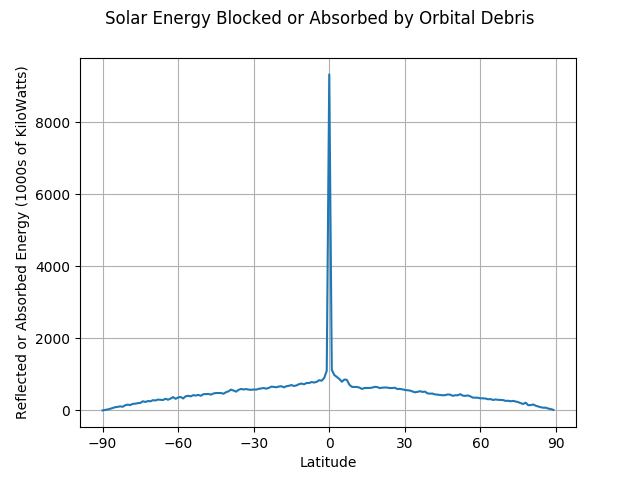
\includegraphics[width=0.75\textwidth]{BlockedSolarEnergy.png}
\label{fig:blockedSunlight}
\end{figure*}
For this research question, it is important to define what is considered significant. How much blocked sunlight is signifigent? And even if the blocked solar energy is "significant" will it have an effect on the climate of our planet? To establish the level of significance a threshold of one-millionth of a percent of the total solar energy received by earth was established. Though this is a tiny number, it represents a considerable amount of energy since the earth receives about 174 petawatts of energy from the sun annually. If the amount of energy blocked is greater than this threshold it will be considered a significant amount, but would most likely not have any effect on temperature or climate on earth since it is such a small percentage. Additionally, if this threshold is passed, the results may be considered inconclusive since it was shown in Section \ref{methods} that the model tends to overestimate the amount of blocked energy.

Based on the calculations made with the model described in Section \ref{methods} the graph shown in Figure \ref{fig:blockedSunlight} was generate. It can be seen that there is a steady increase in blocked energy from higher latitudes to lower latitudes with a large spike at the equator. This large spike is due to a large amount of material sitting in geostationary orbits. Due to the limitations described all these items are represented as blocking sunlight only at the equator. In reality, this blocked energy would be more evenly distributed amount all latitudes. Additionally, the true blocked energy would most likely be much lower than shown in the graph at all latitudes. 

After calculating the total energy blocked by debris as the sum of what is blocked at each latitude, it was found that only 0.000000000052\% of total solar energy received by earth was blocked. This equates to only 52 trillionths of a percent which is far less than our one-millionth of a percent threshold. Therefore, it can be concluded that solar energy does not have a significant effect on insolation even if it does block a large amount of energy.

\subsection{Research Question 2}
The conclusion we can draw for research question 2 stems from the results gathered to answer research question 1. It was concluded that orbital debris does not have a significant effect on insolation. Therefore, it can most reasonably be assumed that orbital reflectors are not a reasonable means to curb global warming. We have been putting things into space for over seventy years. During that time we have been unable to come close to having a noticeable effect on insolation. Since in seventy years we have failed to make any real difference in insolation, it would be foolish to imagine we could make a large enough difference shortly to slow the pace of global warming. One might make the point that during the past seventy years we have not been explicitly trying to block insolation and if we only make a consorted effort, we will be able to make a difference. With this, I disagree. Making a real difference will require the development of new technologies in both rocket and satellite technology. Would it not be better to spend that time, money, and effort developing real solutions to global warming here on earth. It makes far more sense to spend time trying to truly solve the issue instead of reducing the effects. 

\section{Future Work and Conslusion} \label{conclusion}
As stated in Section \ref{methods} there are many limitations with the current model. Some of these limitations are rather easy to fix, while others are far more difficult. Though none of the limitations severely impacted the findings of this paper, improving the modeling would allow for further research. Therefore, in the future, the model will be enhanced to deal with debris being on the day and night side of the earth, the periods of transition between day and night, the tilt of the earth, and more complicated orbit types such as sun-synchronous orbits. Once this has been completed, the model can be expanded to examine new problems. For example, this model could be used to look at the amount of heat orbital debris contributes to the upper atmosphere due to the solar energy it receives. Furthermore, it could be expanded to look at not only orbital debris but working satellites as well. This model, after being extended, could continue to provide insights into the processes that are now occurring in our upper atmosphere due to our recent space exploration.

Orbital debris has been a growing problem over the past few decades, and many of the major concerns with it will not be disappearing, but the question over debris' effect on insolation can be answered with some confidence. It does not have a significant. Furthermore, fanciful ideas about orbital mirrors used to reflect sunlight away from our planet to cool it down can be dismissed. It is unreasonable to assume we could accomplish such a feat if we have made no difference in insolation over the past 70 years. The conclusions of this paper do not only reject the idea that debris affects insolation, but also supports the idea that global warming is an issue that must be dealt with here on earth and not up in orbit.

\end{multicols*}


\end{document}
